\documentclass[11pt, oneside]{article} 
\usepackage{geometry}
\geometry{letterpaper} 
\usepackage{graphicx}
	
\usepackage{amssymb}
\usepackage{amsmath}
\usepackage{parskip}
\usepackage{color}
\usepackage{hyperref}

\graphicspath{{/Users/telliott/Github/calculus_book/png/}}
% \begin{center} 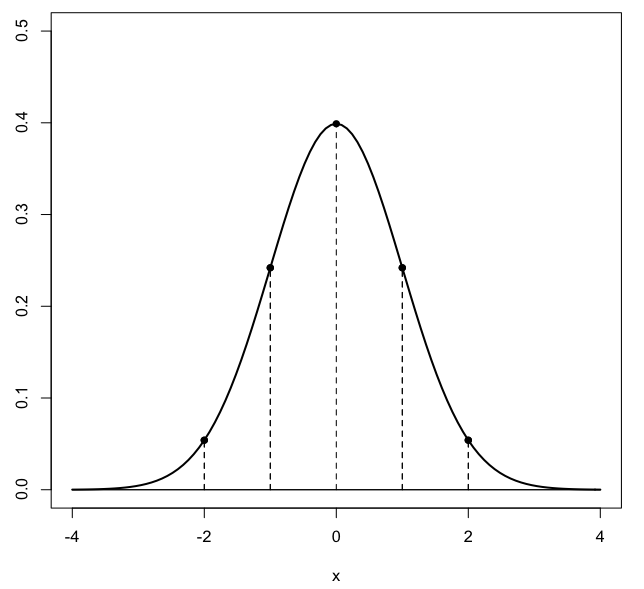
\includegraphics [scale=0.4] {gauss3.png} \end{center}

\title{Sum of squares}
\date{}

\begin{document}
\maketitle
\Large

\begin{center} 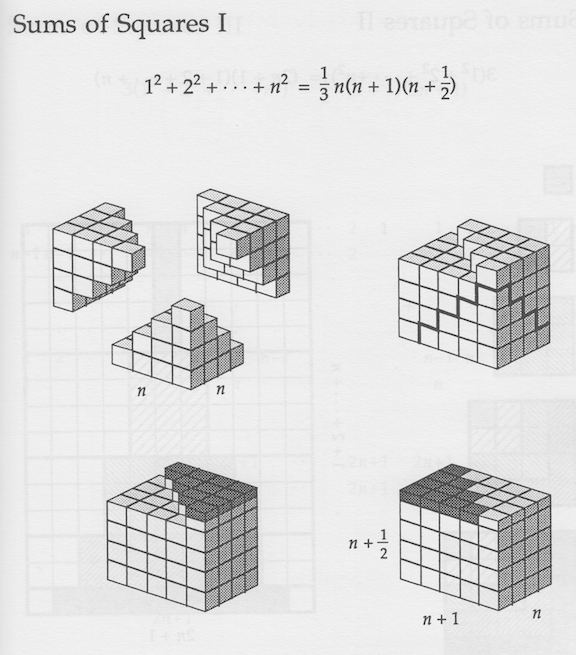
\includegraphics [scale=0.35] {sum_n2.png}\end{center}

We want to find a formula for the sum of the squares of the first $n$ integers.  We briefly discussed how to do this in an earlier chapter.  

The result is
\[ S_n = \sum_{k=1}^n k^2 = \frac{1}{3} \ n(n + \frac{1}{2})(n + 1) \]

This formula is also written variously as
\[ \frac{n(n+1)(2n+1)}{6} \]
\[ \frac{1}{6} \ (2n^3 + 3n^2 + 2n) \]
\[ \frac{n^3}{3} + \frac{n^2}{2} + \frac{n}{3} \]
But I find it easiest to remember the first version.

We can check it by induction.  The base case is easy
\[ \frac{1(2)(3)}{6} = 1 \]  

Now for the induction step:
\[ \frac{n(n+1)(2n+1)}{6} + (n+1)^2 \]
\[ = \frac{n+1}{6}  \ [ \ (n)(2n+1) + 6(n+1) \ ] \]
Look at what's in the brackets
\[ (n)(2n+1) + 6(n+1) \]
\[ = 2n^2 + 7n + 6 \]
\[ = (n + 2)(2n + 3) \]
\[ = (n + 1 + 1)(2(n + 1) + 1) \]
So altogether we have
\[ = \frac{(n+1)(n + 1 + 1)(2(n + 1) + 1)}{6} \]
which indeed, is the formula we had above, substituting $n+1$ for $n$.

$\square$

\subsection*{Derivation by collapsing sum}
Determine the formula for
\[ S_n = 1^2 + 2^2 + \dots n^2 \]

We proceed as we did in the case of the sum of integers.  There we used $(k+1)^2$ and worked out the consequences.  Here we use

\[ (k+1)^3 = k^3 + 3k^2 + 3k + 1 \]
\[ \sum_{k=1}^n (k+1)^3 = \sum_{k=1}^n k^3 + \sum_{k=1}^n 3k^2 + \sum_{k=1}^n 3k + \sum_{k=1}^n 1 \]

Moving the first term from the right-hand side to the left, we obtain a telescoping sum as the difference, just like before:

\[ (n + 1)^3 - 1 = \sum_{k=1}^n 3k^2 + \sum_{k=1}^n 3k + \sum_{k=1}^n 1 \]
Now it's just some messy algebra.  The second term on the right-hand side includes our previous result:
\[ n^3 + 3n^2 + 3n = 3 \sum_{k=1}^n k^2 + 3 \ \frac{n(n+1)}{2} + n \]
\[ 6 \sum_{k=1}^n k^2 = 2(n^3 + 3n^2 + 3n) - 3n(n+1) - 2n \]
\[ 6 \sum_{k=1}^n k^2 = n \ [ \ 2(n^2 + 3n + 3) - 3(n+1) - 2 \ ]  \]
\[ 6 \sum_{k=1}^n k^2 = n \ [ \ 2n^2 + 3n  + 1 \ ]  \]
\[ 6 \sum_{k=1}^n k^2 = n \ (n + 1)(2n + 1) \]
\[ \sum_{k=1}^n k^2 = \frac{n \ (n + 1)(2n + 1)}{6} \]
which can be re-written in various ways including:
\[ \sum_{k=1}^n k^2 = \frac{1}{3} \cdot n (n + 1)(n + \frac{1}{2}) \]

\subsection*{Strang's proof}
Here is another approach, from Strang's \emph{Calculus}.  He says "the best place to start is a good guess".  So again, our goal is to find a formula for:

\[ S = \sum_{k=1}^{n} \ k^2 \]

Perhaps we visualize a pile of cannonballs
\begin{center} 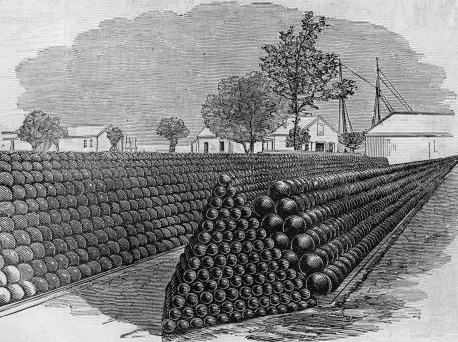
\includegraphics [scale=0.5] {cannonballs.png} \end{center}

Each layer contains a square number of cannonballs ($1$, then $4$, then $9$, etc.).  The shape is a pyramid with dimensions $n \times n \times n$.  We know the formula for the volume of a pyramid, and guess

\[ S_n = \frac{1}{3} n^3 \]

To test it, check whether this difference is $n^2$ (as it should be):

\[ S_{n} - S_{n-1} = \frac{1}{3} n^3 - \frac{1}{3} (n-1)^3 \]

Now

\[ (n-1)^2 = n^2 - 2n + 1 \]
\[ (n-1)^3 = (n-1)(n^2 - 2n + 1) \]
\[ = n^3 - 3 n^2 + 3 n - 1\]

So

\[ S_{n} - S_{n-1} = \frac{1}{3} (n^3 - n^3 + 3 n^2 - 3 n + 1) \]

We see that our guess is off by the residual terms

\[ \frac{1}{3} (3 n^2 - 3 n + 1) \]
\[ = n^2 - n + \frac{1}{3} \] 

Strang says:  the guess needs \emph{correction terms}.  
To cancel $1/3$ in the difference, subtract $n/3$ from the sum.  And to add back $n$ in the difference, add back $1 + 2 + \dots + n(n+1)/2$ to the sum.  Our new guess is

\[ S_n =  \frac{1}{3} n^3 + \frac{n(n+1)}{2} - \frac{n}{3} \]
\[ = \frac{n}{6} (2n^2 + 3(n+1) - 2) \]
\[ =  \frac{n}{6} (2n + 1)(n + 1) \]
\[ = \frac{n(n+1)(2n+1)}{6} \]

which may be easier to remember as

\[ S_n = \frac{n(n+1)}{2} \cdot \frac{2n + 1}{3} \]

\end{document}  